%% Overleaf			
%% Software Manual and Technical Document Template	
%% 									
%% This provides an example of a software manual created in Overleaf.

\documentclass{ol-softwaremanual}

% Packages used in this example
\usepackage{graphicx}  % for including images
\usepackage{microtype} % for typographical enhancements
\usepackage{listings}
% \usepackage{minted}    % for code listings
\usepackage{amsmath}   % for equations and mathematics
\usepackage[final]{pdfpages}
% \usepackage{geometry}
% \setminted{style=friendly,fontsize=\small}
% \renewcommand{\listoflistingscaption}{List of Code Listings}
\usepackage{hyperref}  % for hyperlinks
\usepackage{cleveref}
% \usepackage{markdown}
\usepackage[smartEllipses]{markdown}

\usepackage[a4paper,top=2cm,bottom=2cm,left=2cm,right=2cm]{geometry} % for setting page size and margins

% Custom macros used in this example document
\newcommand{\doclink}[2]{\href{#1}{#2}\footnote{\url{#1}}}
\newcommand{\cs}[1]{\texttt{\textbackslash #1}}
% \geometry{paperheight=22cm, paperwidth=10cm}

\lstset{
numbers=left, 
numberstyle= \tiny, 
keywordstyle= \color{ blue!70},commentstyle=\color{red!50!green!50!blue!50}, 
frame=shadowbox, 
} 

% \lstset{numbers=left, numberstyle=\tiny, keywordstyle=\color{blue!70}, commentstyle=\color{red!50!green!50!blue!50}, frame=shadowbox, rulesepcolor=\color{red!20!green!20!blue!20},escapeinside=``, xleftmargin=2em,xrightmargin=2em, aboveskip=1em}

% Frontmatter data; appears on title page
\title{Hyperparameter Tuning for Milvus via HOBO}
% \version{2.3.1}
\author{Xiang Pan}
% \softwarelogo{
\includegraphics[width=8cm]{logo}}

\begin{document}

\maketitle

\tableofcontents
% \listoflistings
\newpage

\section{Introduction}


For solving the optimization of milvus hyperparameters, we use the Bayesian Optimization and Hyperband(BOHB)\cite{falkner__BOHBRobustEfficient} as our parameter search method.

\section{Methods}
There are several level hyperparameters in milvus, including index-type, index-params and search-params.
To get an end-to-end solution for index, we use BOHB in different level. For Index Type, to eminent the randomness of BO for index-type(which means BO may not fully explore some specific type due to init poor performance), we set two index type optimization mode(Loop and BO).

\begin{figure}[!hpt]
    \centering
    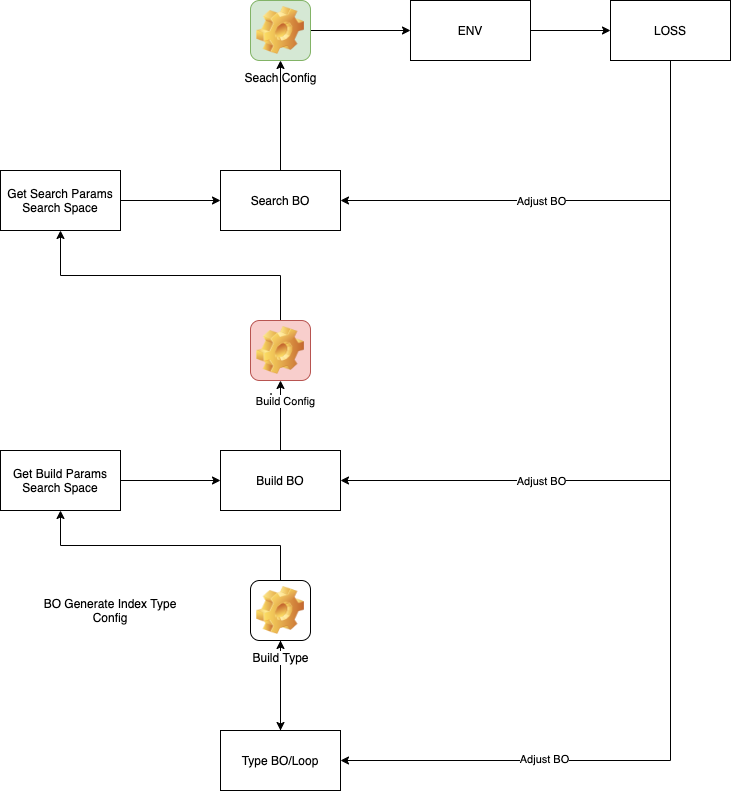
\includegraphics[width=0.9\textwidth]{../figures/flow.png}
    \caption{\label{fig:flow}Flow Diagram}
\end{figure}

\subsection{Loss Function}

We use laplace method to convert constraint BO to unconstraint version.
Our loss function is as below:  
\begin{align}
Loss = sign(recall, threshold) - query\_per\_sec 
\end{align}


\begin{align}
Sign(recall, threshold) = 
\begin{cases}  
recall - threshold & recall>threshold \\
\lambda * (threshold - x) & recall<=threshold,
\end{cases}
\end{align}

Here we use $\lambda = 100000$ for Lagrange method, and $threshold = 95$.

\section{Implemtation}
\subsection{Hardware Information}
Our method is tested on server with:
CPU: Intel Core i7-8700 CPU @ 4.6GHz and 
RAM: 32083MiB.

\subsection{Core Code Annotations}
\subsubsection{ENV}

ENV is a helper class configure basic milvs related variables. 
\begin{lstlisting}[language=python,numbers=left,basicstyle=\footnotesize, caption={ENV class config}] ]
class ENV():
def __init__(self, args = None):
    print("ENV")
    # docker related information
    host = '127.0.0.1' 
    port = '19530'

    # get milvus client and collection_name
    self.client = Milvus(host, port)
    self.collection_name = args.collection_name
    
    # get query_vectors and set top_k
    self.query_groundtruth = self.get_groundtruth()
    self.query_vectors = self.get_query()
    self.top_k = 100

    # get status by curretn db 
    self.index_type = None
    self.index_params = None
    self.refresh_status()

    # set datadim, which is needed by some serch constraint
    global gDataDim
    gDataDim = 128

    # based on the input type, get the default build config
    if args.op == "build_params":
        self.target_index_type = get_index_type(args.index_type)
        self.target_index_params = \ 
        get_default_build_config(self.target_index_type)

        is_build = False
        if self.index_type != self.target_index_type:
            is_build = True
        elif self.index_params != self.target_index_params:
            is_build = True
        
        if is_build:
            self.env_build_input(self.target_index_type,\
                self.target_index_params)
            self.refresh_status()

    # set search space
    self.default_build_config = get_default_build_config(self.index_type)
    self.search_configspace = get_search_configspace(self.index_type,\ 
        self.index_params)
    self.build_configspace = get_build_configspace(self.index_type)
\end{lstlisting}

\begin{lstlisting}[language=python,numbers=left,basicstyle=\footnotesize, caption={Refresh Status}]
# base on user's input, get the target search space
def refresh_status(self):
    """
    refresh status
    reset index_type and index_params
    reset all config space 
    """        
    status, stats = self.client.get_index_info(self.collection_name)
    self.index_type = stats._index_type
    self.index_params = stats._params

    # set config space
    self.default_build_config = get_default_build_config(self.index_type)
    self.build_configspace = get_build_configspace(self.index_type)
    self.search_configspace = get_search_configspace(self.index_type,\ 
        self.index_params)
\end{lstlisting}



\subsubsection{Search Config Class}
\begin{lstlisting}[language=python,numbers=left,basicstyle=\footnotesize, caption={Search Config Class}]
class HNSW_build_search_shared_config(object):
def __init__(self):
    self.M =  cs.IntegerUniformHyperparameter('M', 4, 64)
    self.efConstruction =  \ 
        cs.IntegerUniformHyperparameter('efConstruction', 8, 512)
    top_k = 100 
    self.ef =  cs.IntegerUniformHyperparameter('ef', top_k, 512)          
    self.configspace = \ 
    cs.ConfigurationSpace([self.M, self.efConstruction, self.ef], seed=123)
\end{lstlisting}
We use constant class to configure the default search space.


\subsubsection{ENV Input}
\begin{lstlisting}[language=python,numbers=left,basicstyle=\footnotesize, caption={Input}]
# given full env put
def config_input(self, config):
    # check current index type
    is_build = False

    self.refresh_status()
    if self.index_type != config['index_type']:
        is_build = True
    elif self.index_params != config['index_params']:
        is_build = True
    
    if is_build:
        self.env_build_input(config['index_type'] ,config['index_params'])
        self.refresh_status()
    

    recall, query_per_sec = self.env_search_input(config['search_params'])
    self.search_params = config['search_params']
    
    return recall, query_per_sec
\end{lstlisting}
For input, we check the current status and mark the change that need to be done. Once we have changed the index of current database, we refresh the ENV status.


\subsection{User Input Parser}
\begin{lstlisting}[language=python,numbers=left,basicstyle=\footnotesize, caption={Input Parser}]
if args.op == "build_type":
    build_type_search_spcae =\ 
    [IndexType.IVF_FLAT, IndexType.IVF_PQ, IndexType.IVF_SQ8, IndexType.HNSW]
    if args.build_type_op_method == "BO":  # BO
        index_type = \ 
        cs.CategoricalHyperparameter('index_type', build_type_search_spcae)
        index_type_configspace = cs.ConfigurationSpace([index_type], seed=123)
        type_opt = \ 
        BOHB(index_type_configspace,\
         build_type_evaluate, max_budget=10, min_budget=1)
        type_logs = type_opt.optimize()
    else:                                 # Loop
        for index_type in build_type_search_spcae:
            env.target_index_type = index_type
            env.refresh_status()
            opt = \
            BOHB(get_build_configspace(env.target_index_type), \ 
            build_evaluate, max_budget=10, min_budget=1)
            logs = opt.optimize()
\end{lstlisting}

The input parser is trival.

\newpage
\subsection{HOBO}
\begin{lstlisting}[language=python,numbers=left,basicstyle=\footnotesize, caption={HOBO}]
# Based on the HOBO class and our search space configuration, \ 
# we can build a BOHB object. After that, we can call the optimize() \ 
# method to start the optimization process.
def build_type_evaluate(params, n_iterations):
env.target_index_type = params['index_type']
env.refresh_status()
if args.build_search_share_space:
    opt = BOHB(get_build_search_shared_configspace(env.target_index_type),  
                build_search_share_space_evaluate, 
                max_budget=n_iterations, 
                min_budget=1, 
                eta = 10)
    logs = opt.optimize()
else:
    opt = BOHB(get_build_configspace(env.target_index_type), 
                build_evaluate, 
                max_budget=n_iterations, 
                min_budget=1,  
                eta = 10)
    logs = opt.optimize()
return logs.best['loss']
\end{lstlisting}

\newpage
\section{Results}
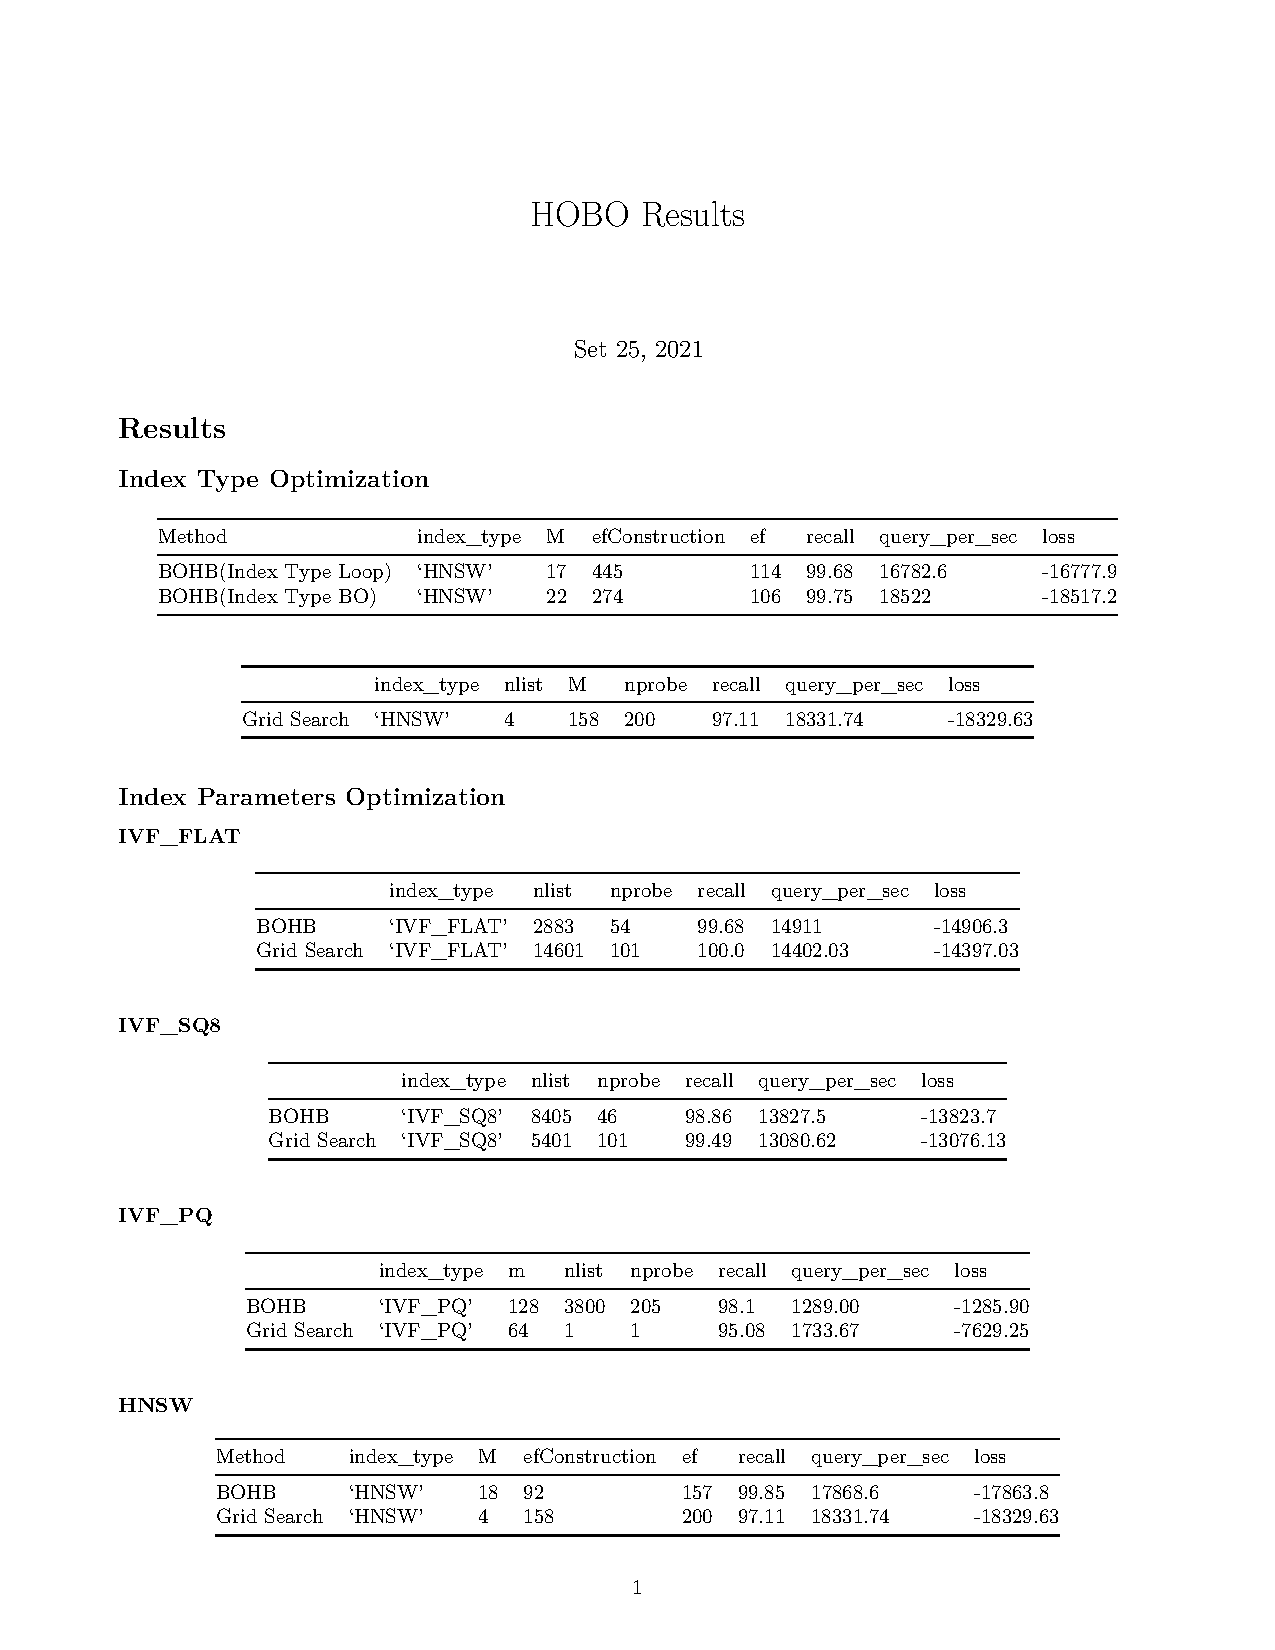
\includepdf{table.pdf}

\section{Attemption}
\subsection{VAE}


Trying to conpress the embedding dimension and get a more milvus-friendly representation space, we are using VAE to preprocess the given datasets.


\subsubsection{Measure of Rank keeping}
We define the overlap and exact-match to measure the rank-keeping performance.
\begin{align}
    overlap = \frac{1}{|D|} \sum_{eb \in D} \frac{\text{knn of f(eb)} \cap \text{knn of eb}}{\text{knn of eb}}
\end{align}

\begin{align}
    overlap = \frac{1}{|D|} \sum_{eb \in D}  \frac{\sum_{neb\in \text{neibor of eb}}\text{rank f(neb)} == \text{rank of neb}}{k}
\end{align}

\subsubsection{Methods}

\textbf{Minimum Reconstruct Error}

\begin{align}
    Loss_{MRE}(eb) = decoder(encoder(eb)) - eb
\end{align}

We use $compressed\_eb = encoder(eb)$ for milvus search.

\textbf{Distance Preserving}
\begin{align}
    Loss_{RP}(e1, e2) = \|e1 - e2)\|_2 - \|encoder(e1) - encoder(e2)\|_2
\end{align}

\textbf{Contrastive Learning}
The key idea of contrastive learning is to use contrastive loss to make the embedding keep the relative distance, which "may" be useful for keeping the rank.
\begin{align}
    Loss_{CL}(a, p, n) = \|a - p\|_2 - \|a-n\|_2
\end{align}
Similarly, we have,
\begin{align}
    Loss_{CL}(a, p, n ,f) = \|f(a) - f(p)\|_2 - \|f(a)-f(n)\|_2
\end{align}
f is the encoder function.

For a, p and n, a is the anchor, p is the positive and n is the negative. Positive and negative can be decided by their relative distance.
\begin{itemize}
    \item If p is closer to a than n, then p is positive and n is negative.
    \item If p is top-k nearest neighbors of a but n is not, then p is positive and n is negative.
\end{itemize}

Our empricial result is that the loss of contrastive learning and vae can not preserving the relative distance rank between embedding. 

\subsection{Graph Based Message Passing}
We use message passing to make the more similar embedding closer. First, we build the knn graph $g$ for given dataset $D$. Over graph g, we define the following message passing function, 

\begin{align}
    u' = u + reduction(aggregation(v, e))
\end{align}

For each node u in g, v is their neighbors, e is the edge between u and v, and aggregation is the aggregation function.

We use $aggregation=e\_mul\_v$ and $reduction\in\{mean,max,min,sum\}$. The result shows that max get the best performance, which may suggest that simply average the neighbors' embedding is not enough. However, the best overlap performance is around 0.65, which is not good enough for ranking preserving.

\subsection{Minimum Distortion Embedding}
We use the method proposed in \cite{agrawal__MinimumDistortionEmbedding}, which is to minimize the distortion of embedding rank while comperssing the embedding dimension. 




% \subsection{How to create Sections and Subsections}

Simply use the section and subsection commands, as in this example document. With Overleaf, all the formatting and numbering is handled automatically according to the template you've chosen. If you're using Rich Text mode, you can also create new section and subsections via the buttons in the editor toolbar.

\subsection{How to include Figures}

First you have to upload the image file from your computer using the upload link in the file-tree menu. Then use the includegraphics command to include it in your document. Use the figure environment and the caption command to add a number and a caption to your figure. See the code for Figure \ref{fig:frog} in this section for an example.

Note that your figure will automatically be placed in the most appropriate place for it, given the surrounding text and taking into account other figures or tables that may be close by. You can find out more about adding images to your documents in this help article on \href{https://www.overleaf.com/learn/how-to/Including_images_on_Overleaf}{including images on Overleaf}.

\begin{figure}
\centering
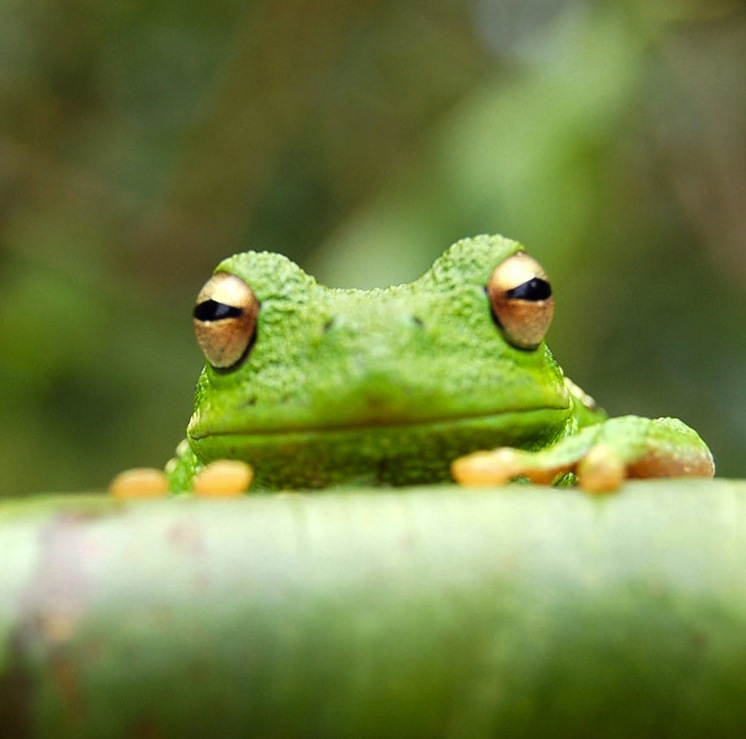
\includegraphics[width=0.3\textwidth]{frog.jpg}
\caption{\label{fig:frog}This frog was uploaded via the file-tree menu.}
\end{figure}

\subsection{How to add Tables}

Use the table and tabular environments for basic tables --- see Table~\ref{tab:widgets}, for example. For more information, please see this help article on \href{https://www.overleaf.com/learn/latex/tables}{tables}. 

\begin{table}
\centering
\begin{tabular}{l|r}
Item & Quantity \\\hline
Widgets & 42 \\
Gadgets & 13
\end{tabular}
\caption{\label{tab:widgets}An example table.}
\end{table}

\subsection{How to add Comments and Track Changes}

Comments can be added to your project by highlighting some text and clicking ``Add comment'' in the top right of the editor pane. To view existing comments, click on the Review menu in the toolbar above. To reply to a comment, click on the Reply button in the lower right corner of the comment. You can close the Review pane by clicking its name on the toolbar when you're done reviewing for the time being.

Track changes are available on all our \doclink{https://www.overleaf.com/user/subscription/plans}{premium plans}, and can be toggled on or off using the option at the top of the Review pane. Track changes allow you to keep track of every change made to the document, along with the person making the change. 

\subsection{How to add Lists}

You can make lists with automatic numbering \dots

\begin{enumerate}
\item Like this,
\item and like this.
\end{enumerate}
\dots or bullet points \dots
\begin{itemize}
\item Like this,
\item and like this.
\end{itemize}

\subsection{How to write Mathematics}

\LaTeX{} is great at typesetting mathematics. Let $X_1, X_2, \ldots, X_n$ be a sequence of independent and identically distributed random variables with $\text{E}[X_i] = \mu$ and $\text{Var}[X_i] = \sigma^2 < \infty$, and let
\[S_n = \frac{X_1 + X_2 + \cdots + X_n}{n}
      = \frac{1}{n}\sum_{i}^{n} X_i\]
denote their mean. Then as $n$ approaches infinity, the random variables $\sqrt{n}(S_n - \mu)$ converge in distribution to a normal $\mathcal{N}(0, \sigma^2)$.

\subsection{How to customize the template}

You may wish to customize the template for your own style, or to meet the specific needs of your documentation. If you're already familiar with LaTeX,  you can go ahead and add the packages you're familiar with to the document preamble. If you run into any problems and can't find the answers in the package documentation or in the Overleaf \doclink{https://www.overleaf.com/learn}{help library}, the forums such as \doclink{https://tex.stackexchange.com/}{TeX StackExchange} and \doclink{https://latex.org/forum/}{LaTeX Community} are a great source of answers.

Some details on how to customize a .cls file (which sets the layout and overall format of the various elements of the template) can be found at \doclink{https://www.overleaf.com/learn/latex/Writing_your_own_class}{Writing your own class}, and \doclink{http://texdoc.net/pkg/clsguide}{\LaTeX2e\ for class and package writers}. 


\bibliographystyle{plain}
\bibliography{main}

\end{document}
